


\documentclass[journal]{IEEEtran}

\hyphenation{op-tical net-works semi-conduc-tor}
\usepackage{float}
\usepackage{graphicx}
\usepackage{subcaption}
\usepackage{xcolor}

\newcommand{\specialcell}[2][c]{%
  \begin{tabular}[#1]{@{}c@{}}#2\end{tabular}}

\usepackage[utf8]{inputenc}

\usepackage[unicode]{hyperref}
\hypersetup{
    colorlinks=true,
    linkcolor=blue,
    filecolor=magenta,      
    urlcolor=cyan,
    pdftitle={Overleaf Example},
    pdfpagemode=FullScreen,
    }
\urlstyle{same}

 
\begin{document}

\title{Final Project Report\\ Mushroom Identification}


\author{Tim Lu, \textit{BNN}; Allen Liao, \textit{CNN}; Mikayla Krech, \textit{DINOv2ViT}; and Namith Rao, \textit{LDA}
}



% The paper headers
\markboth{Journal of Computational Mycology,~Vol.~14, No.~10, December~2024}%
% \markboth{Journal of \LaTeX\ Class Files,~Vol.~14, No.~8, August~2015}%
{Shell \MakeLowercase{\textit{et al.}}: Bare Demo of IEEEtran.cls for IEEE Journals}



% make the title area
\maketitle

% As a general rule, do not put math, special symbols or citations
% in the abstract or keywords.
\begin{abstract}
In this paper we examine the highly challenging task of mushroom identification as well as the major hurdles associated with this task. Through our research, we have found a number of papers that broach the subject of mushroom identification although a common thread among these papers remains and that is \textit{mushroom identification is hard}. As one might expect, a problem as difficult as this leaves open a number of valid and unproven strategies such as Vision Transformers, CNN, LDA, Bayesian Neural Network, and pre-trained image segmentation models on the mushroom identification problem. In a sense, we went ''full circle''with our paper as our experimental results, with a max validation accuracy of 71.52 percent, confirm what the limitations of image based mushroom identification and our methods.
\end{abstract}

% Note that keywords are not normally used for peerreview papers.
\begin{IEEEkeywords}
Computer Vision, Mycology, Image Processing, Image Segmentation, CNN, BNN, DINO, Vision Transformer, LDA, Classifier.
\end{IEEEkeywords}




\IEEEpeerreviewmaketitle



\section{Introduction}

\IEEEPARstart{T}{}he humble mushroom is a familiar sight at almost any grocery store, marked by its characteristic cap, gills, stalk, and a typically brownish/whitish hue \textit{(in the case of Cremini and Portabello mushrooms)}. These said mushrooms are fairly non-distinct in appearance and have earned the moniker of "garden variety", however the reality is that these mushrooms only represent a small sliver of the total types of mushrooms in the world. Moreover, old methods of visually identifying mushrooms that might have worked with "garden variety" mushrooms quickly falls apart fast in the real world because the edibility of a mushroom cannot be generalized from how much a mushroom looks like it came from a grocery store shelf. In fact, the problem of visually identifying mushrooms based on appearance can fall apart so fast in real world applications that sometimes the recommendation is to abandon visual identification altogether in favor of spore print and chemical analysis due to poisonous look-alikes \cite{groves1979mushrooms}.
Nonetheless, identifying mushrooms with the application of computer vision techniques is a highly relevant subject today. With the use of computer vision techniques, the aim of our project is to identify mushrooms from images which would normally take expert training and qualifications thereby breaking a certain skill ceiling. Additionally, our project aims to be able to visually identify psychedelic/hallucinogenic mushrooms as current mushroom identification apps do not seem to support this feature.



\section{Relevant Literature}
Presently, much of the computer vision literature on mushrooms is closely tied with the needs of the agricultural industry. As one would expect, there is a very practical need for more efficient methods of mushroom identification in the field of mushroom farming, and consequently much of the research is driven around improving mushroom crop yields. To name a few of the leading areas of mushroom related research in computer vision, work has been done on estimating the 3D pose of a mushroom using point clouds, and additionally, CNN based methods for mushroom quality estimation have also shown promise.
\par
In addition to deep learning techniques, we reviewed literature that used different methods for image classification. This includes usage of PCA and LDA as a classifier \cite{lakshika2021}. This paper uses computer vision techniques to extract interpratable features from leaf images in order to classify them. The authors describe a seven-step preprocessing pipeline including RGB, grayscaling, gaussian smoothing, binary thresholding, and segmentation. They extract 52 features categorized by shape, color, texture, and scagnostic based features. After processing, they use PCA and LDA for dimensionality reduction and feature space visualization. It was found that PCA and LDA were effective in distinguishing between plant species, and showed a clear separation between classes. This can be applied to the problem of mushroom classification, from preprocessing to feature extraction, and dimensionality reduction.
\par
It should also be noted that while much of the literature is constrained to edible mushrooms only, a great many number of visual features and identifiers are sough after in mushroom identification. Examples of different mushroom identification methods can be found on the table on the top of the second page.


\begin{figure*}
    \centering
    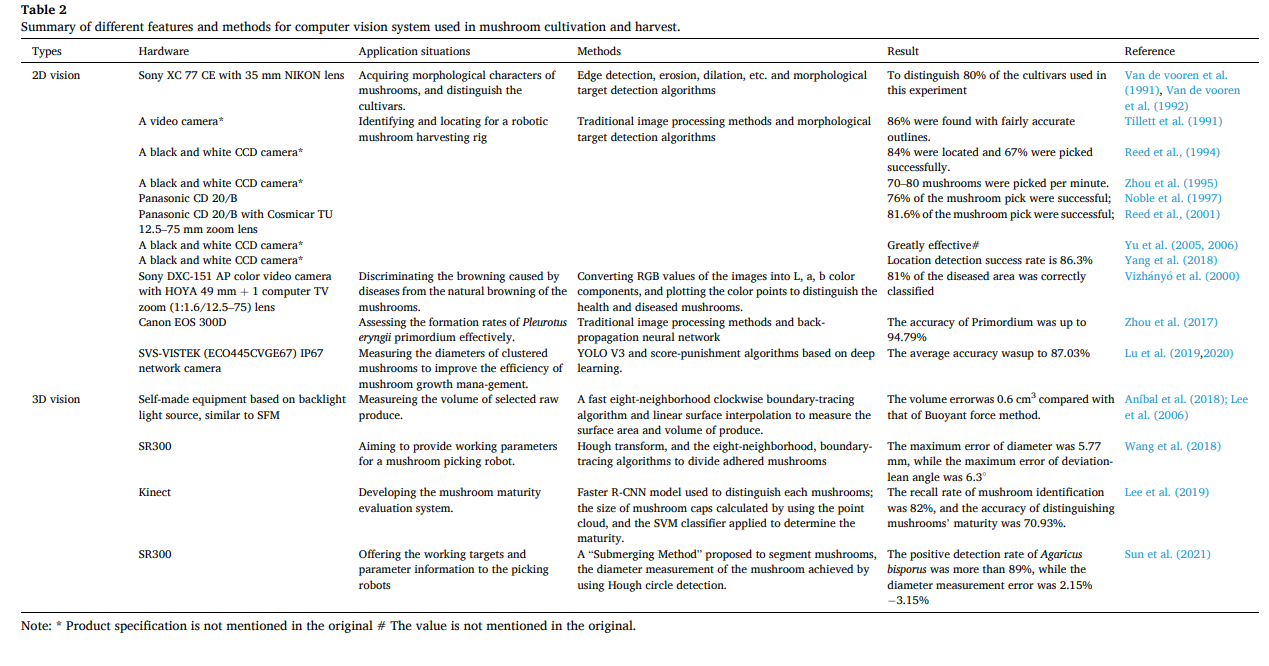
\includegraphics[width=\textwidth,height=7cm]{imgs/mushroom_methods.PNG}
    \caption{Mushroom Literature. \cite{10.1016/j.compag.2022.107015}}
    \label{fig:Mushroom Literature}
\end{figure*}


\section{Dataset}
As stated in our project proposal, we used the FGVCx dataset \cite{fungi-challenge-fgvc-2018}, created for the 2018 FGVCx Fungi Classification Challenge \cite{Visipedia}. It consisted of 85,578 training and 4,182 validation images of 1394 different species. Since it does not have labels for poisonous or edible mushrooms, we had obtain that information elsewhere. We found a website with data on poisonous and edible mushrooms. Although the website does not have an API, we were able to parsed it with a scraper and labeled our images with poisonous or edible, based on the species label that comes with the FGVCx dataset. This reduces our dataset to about 50,312 training and 1,773 validation images of 591 species. The training split was 64.75\% edible mushrooms and the validation split was 61.59\% edible mushrooms, so there is only a slight skew.
,


\section{BNN}
As alluded to earlier in the abstract, mushroom identification is hard but this still requires more explanation. Before mushroom identification can begin an important precondition is determining whether there is a mushroom present in the image but that requires knowledge of the mushroom’s appearance. For simplicity, this project assumes (unrealistically) that there must always be a mushroom in the image but this precondition naturally brings to mind a very relevant question: what should mushrooms look like?


A question as simple sounding as this should be relatively straightforward but the reality is far different. While many mushrooms have the ''umbrella'' shape, a significant number of mushrooms have forms that radically differ from this and thus any classification approaches based on the classic ''umbrella'' shape must go out the window. Since it is factually impossible to generalize mushroom appearances, another good alternative is to pick up as many identifiable features from the mushroom as possible and use a Bayesian Neural Network (BNN) approach to generate probabilistic estimates.

The BNN approach can be thought of as a natural extension of Baye's rule. In the BNN, the architecutre of the network can be represented as a directed acylic graph where the direction of the arrows determines the conditional relationships between variable or categorical features of mushrooms in our case. Using maximum-likelihood estimation, the conditional probabilities are calculated and ultimately a probablistic estimate of mushroom edibility can be generated. With our network, the simplest possible BNN graph was used in which all the nodes representing common categorical mushroom features are assumed independent.    

While the BNN generates the final probablistic estimate from categorical mushroom features, several interconnected steps must come beforehand to transform an image of a mushroom into categorical features the BNN can process. The pipeline begins with  pre-trained Yolov11 and FASTSAM models that are used to identify and segment mushrooms from images. Next, a ResNetv18 architecture is trained on a custom dataset of approximately 800 mushroom images. Each image is labeled with physical descriptions in a CSV-style format, covering five of the most common mushroom features: \textit{ cap-shape, cap-surface, gill-attachment, gill-spacing, and gill-size}. In parallel, PCA is applied to the processed images to extract the \textit{cap-color} feature. Together, the ResNet and PCA produce all six categorical features required for BNN classification, enabling the probabilistic estimation of mushroom characteristics and edibility.


\section{DINOv2ViT}
\subsection{Motivation for Model Choices}
My motivation for using a vision transformer (ViT) is not only because they are a common tool used and I am somewhat more familiar with transformers due to my work in linguistics but also because they move beyond convolutional architectures to process images as sequences of patches \cite{ViT}. This structural innovation allows ViTs to capture long-range dependencies within an image, a critical capability for recognizing subtle features, which is especially important for us in distinguishing poisonous from edible mushrooms. ViTs can inherently model global contextual relationships, unlike other convolutional networks, such as the interaction between mushroom cap texture and gill structure.

That said, one of the primary challenges in mushroom identification we discovered (not only in the literature but through our own experience of searching) is the lack of extensively labeled datasets that accurately distinguish between images of poisonous and edible species. 

Traditional supervised methods, including standard ViTs, are constrained by the need for annotated data, which is labor-intensive and time-consuming. DINO, a self-supervised learning framework, provides a great alternative by making use of data with no labels. It enables the model to learn the semantic features of the mushrooms, such as the texture and cap morphology, without requiring manual annotations. This self-distillation approach aligns well with the project's goal of identifying toxic mushrooms in real-world scenarios with sparsely labeled datasets. However, in implementing my model, I did not fine-tune the backbone or attempt to train the model while restricting the model’s access to the labels. This choice was partly to keep my results comparable to my group member’s work and make the model easier for me to implement, as I am still relatively unfamiliar with this process.  

The use of DINO is even more promising for our mushroom classification task because it facilitates the emergence of meaningful visual representations \cite{DINOv2}. These representations, which are visible in self-attention maps, intrinsically highlight significant visual features in an image or image patch, such as object boundaries and possible segmentations. Such properties make DINO ideal for fine-grained identification and differentiation between visually similar mushrooms.

\subsection{Specific Implementation Approaches}
Firstly, my DINOv2ViT code is at this \href{https://drive.google.com/drive/folders/1nChekUzE9uQRjtYzLk8Mhjft8VtLLhTx?usp=drive_link}{Google Drive link}. My main file is "vit\_mushroom\_dino\_3.ipynb" and the "Copy of vit\_mushroom\_dino\_3.ipynb" displays the results from the second half of my last run. There are a few draft files for the ViT, but I did not include all of them because there were \textit{a lot}. The "ViT\_weights" folder has the final saved weights from my last training run and, similar to the draft code folder, still has some of the weights from previous runs. Lastly, I included a code to plot our accuracy results in the drive. 

Continuing with the specific approaches and choices I made, I initially tried to implement a basic PyTorch ViT by loading "self.enc = vit\_b\_16(weights=ViT\_B\_16\_Weights.DEFAULT)" from \cite{ViT}. However, after the initial feedback from our first presentation, I planned to implement a DINOv2 vision transformer as it can encode localized semantic information at a high spatial resolution, which increases the amount of information held in each feature of the mushroom image compared to the information held by the pixels themselves \cite{DINOv2}. Therefore, I instead used Facebook Research's "self.enc = torch.hub.load('facebookresearch/dinov2', 'dinov2\_vits14', pretrained = True)" as my model's head. This backbone splits the input images into 14x14 patches. Smaller patches retain more granular details, which is important for identifying texture and gill patterns in mushrooms.

Images were preprocessed by resizing them to 224x224 pixels, which is a standard input size for the ViT architecture we saw frequently in the literature. More straightforward transformations, such as resizing and tensor conversions, were applied, but I did not attempt more advanced augmentations. Training the DINOv2ViT model with pre-trained weights significantly reduced training times per epoch compared to initializing the model from scratch (which I was accidentally trying to do at some points). I used the Adam optimizer with a learning rate of 1e-4. I trained the model for 30 epochs on the high-RAM, T4 Colab connection. To manage computational resources more efficiently, I attempted to implement dataset caching in image loading, which resulted in faster training epochs following the first one. This optimization proved particularly valuable, given the size of the training set.

Adding some detail to that point: I had many things still implemented slightly incorrectly at the time of our last presentation. In trying to fix my implementation, I changed the encoding head of my model to a basic CNN, a basic MLP, and a basic ViT head compared to the DINO head. I did this because the runtime of each training epoch was much slower than my other group members at first. In the last run, after the first training epoch that was caching the image data, the training epochs (including the evaluation of each epoch) took only approximately 10 minutes, which I found perfectly reasonable for a dataset of 50,000 images. So, although my earlier implementations took a ton of time to run due to my own inefficiencies, in testing these different encoders, I found that ViTs are not always used in real-world applications because their runtimes are not very efficient, especially for larger images \cite{ViTSpeeds}. 

In the proposal, I also said I would explore possible model comparison methods, and our group agreed that classification accuracy in the training set and benchmark performance for images not in the training or testing set was a good fit for this project. However, I also explored using \href{https://lightning.ai/docs/torchmetrics/stable/}{TorchMetrics} for accuracy calculation, and I thought it worked well. The only issue I ran into was implementing the evaluation updates in my training function because switching between model.train() mode and model.eval() mode was not going smoothly. That added a chunk of runtime to each epoch as I had to rerun through the dataset for evaluation. Still, there were pros to using that approach over calculating it by hand.  

Further tests that I attempted during my many training runs included experimenting with scheduling learning rates with an exponential function and a step function, weighting the loss functions with a binary cross entropy loss that penalized misclassifying the poisonous mushrooms by the opposite probability of the data split (~64\%), adjusting batch normalization and dropout rates to avoid overfitting, and tuning the number of parameters in the model. By the end, despite attempting many iterations of the code, due to only finding some fundamental errors in implementing my pre-trained head very recently, I ended up removing most of these “refinements” because I did not have the time or compute credits to see which of these options produced the best results properly.



 
 
 
\section{CNN}
A CNN uses convolutional layers to scan the image and learn specific features, like edges, corners, and texture, creating feature maps, then the pooling layers reduce the spatial dimensions of the feature maps while preserving important information. With the assumption that whether a mushroom is poisonous or not can be extrapolated from its visual features (which we later learned that the assumption is likely false––as discussed previously), we presumed that a CNN would be able to classify mushrooms without us identifying the exact visual features that indicates a mushroom is poisonous.
Originally, Resnet50 architecture is used as the CNN. But as training one epoch takes more than $1.5$ hours, Resnet18 is used instead. Imagenet weights are also used, as the model with random weights takes too long to converge. Immediately after the CNN is an MLP with the following layer:
\begin{enumerate}
    \item Flatten
    \item Batch Normalization ($1$ dimensional)
    \item Linear ($512$ to $128$)
    \item ReLU
    \item Dropout ($0.1$ dropout ratio)
    \item Linear ($128$ to $32$)
    \item ReLU
    \item Dropout ($0.1$ dropout ratio)
    \item Linear ($32$ to $1$)
    \item Dropout ($0.1$ dropout ratio)
    \item Sigmoid
\end{enumerate}
The loss is computed using Binary Cross Entropy Loss. The Adam optimizer is used with PyTorch's implementation of L2 Regularization. A step learning rate scheduler is employed with the epoch set to $5$.
I arrived at the above model by iteratively improving it. At first, only the Flatten, Linear, and Sigmoid layers are used (with only one Linear layer), with no regularization nor scheduler. As I added more Linear layers, the model converged quicker, but started showing signs of overfitting. Despite it not performing well on the validation set, its training accuracy can reach $99\%$ in $7$ epochs. So I started adding Layers like Dropout layers (initially with a ratio of $0.2$, then eventually $0.1$), Batch Normalization, step scheduler and weight L2 Regualrization, while also decreasing the initial learning rate. The model eventually converged slower.

\section{LDA}
We also went with an approach to mushroom classification without using neural networks, that would be functional on smaller datasets, as we did not have many resources for datasets online. As described in \cite{lakshika2021}, Linear discriminant analysis with PCA offers a good strategy for classification, especially becuase it retains interpretability that the deep learning approaches above do not. Using the collected dataset, the images are run through a pre-processing pipeline for resizing, segmentation, and edge detection using SAM and canny edge detection. Then, I used pca and lda for dimensionality reduction and classification. PCA reduces the dimensionality of data while keeping the most significant features necessary for classification. I convert the images to a lower-dimensional that captures as much of the variance in the image data as possible. This is then fed into an LDA classifier to futher reduce dimensionality and maximize class separability. It finds a linear combination of features that best separates the classes of edible or poisonous. This method allowed me to bypass the large computational cost of previous solutions, and allowed me to rely on a smaller dataset.
\section{results}
\subsection{BNN results}
Initially, the BNN approach seemed like a very valid method for mushroom classification and during the initial rounds of testing BNN had the highest, by a slim margin, test accuracy of 61\% on the Fungi Challenge dataset. Looking back, while the BNN approach to mushroom identification is much more lightweight and speedy versus CNN or DINO, BNN is operating in a comparatively lower dimensional space limiting its approximation abilities.
\par
Furthermore, unlike other methods, the BNN implementation came from the pgmpy package which unlike pytorch or tensorflow, does not support batch training and therefore the entire training dataset had to be loaded in all at once which lead to concerning signs of overfitting. This difference likely lead to the BNN making the best generalization it could on the entire training dataset instead of learning the true structure and geometry of what makes a mushroom poisonous or safe to eat.
\par
Another point that needs to be be raised about BNN is the oversimplified assumptions made in the BNN model. In the BNN model, six categorical features are taken: cap-color, cap-shape, cap-surface, gill-attachment, gill-spacing, and gill-size, but there are no vertices connecting related features like cap-shape or cap-surface. Assuming complete independence in all likelihood worsened the predictive abilities and as a matter of fact a better BNN model was generated using Hill-climb optimization with inter feature dependencies, however this was never tested in the interest of time.
\par
One final point about the drawbacks of the BNN results is that BNN relies too heavily on image pre-processing and anything not directly related to the mushroom in the image itself could cause problems. PCA was used to generate color estimates on mushrooms as part of the categorical features fed into BNN, but sometimes the segmentation/mushroom detection pipeline failed leading to instances in which a ''red'' mushroom may be mistakenly labelled ''green'' because of the background.
\par
Overall, the results of the BNN are technically ''passing''. The BNN is able to score an accuracy higher than 50\% which surpasses random chance. Moreover, the BNN when tested on the Fungi Challenge dataset could label some mushrooms as poisonous as sometimes our classifiers would completely fail to learn and instead predict every mushroom image as edible. The fact that BNN has ''learned'' the difference between a poisonous and edible mushroom, \textit{although not very well}, is much more telling in the mushroom look-alike benchmark photos. In the benchmark photos composed of mushroom look alikes, BNN predicted the first two pairs as all edible while BNN predicted the last pair of white mushrooms as completely poisonous.

\begin{figure}[ht]
\centering
\begin{subfigure}[b]{0.45\textwidth}
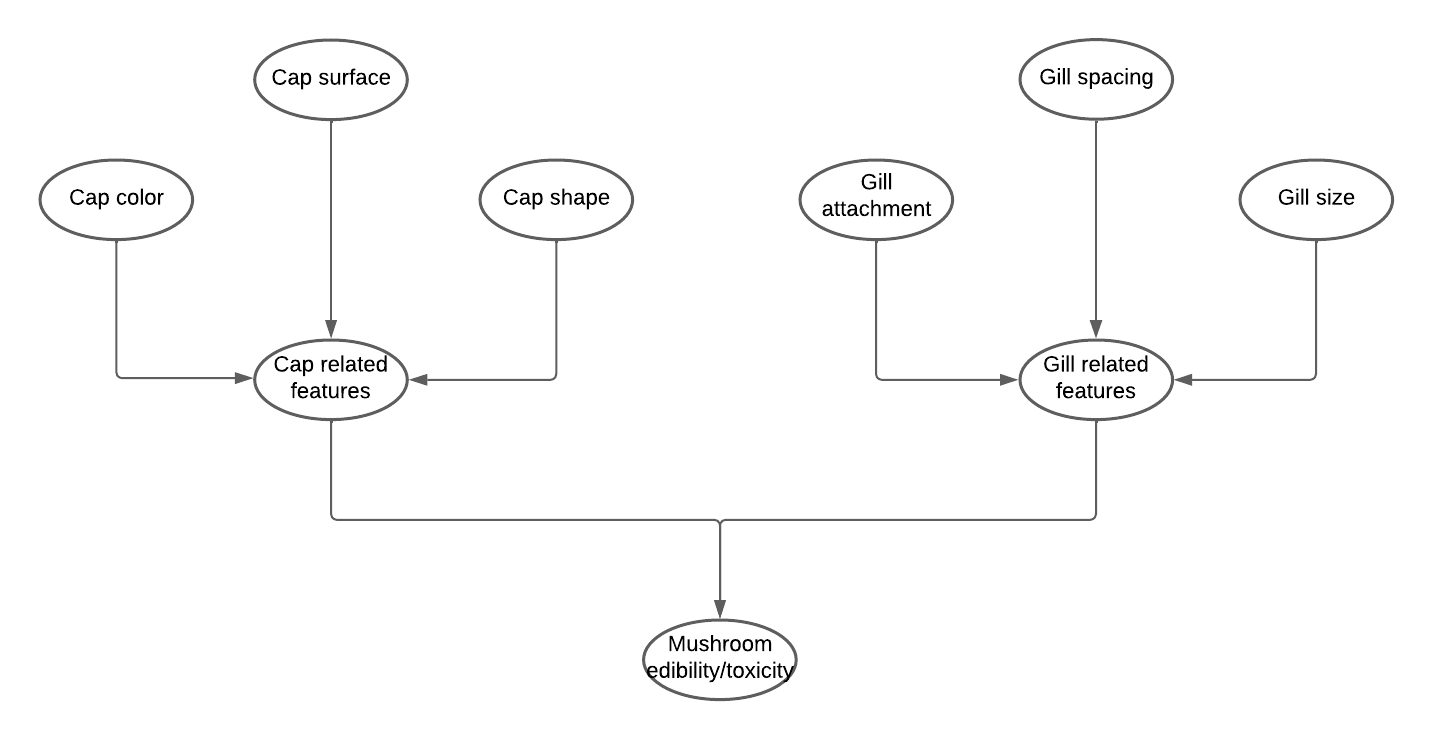
\includegraphics[width=\textwidth]{imgs/DAG.png}
\end{subfigure}
\hfill
\begin{subfigure}[b]{0.45\textwidth}
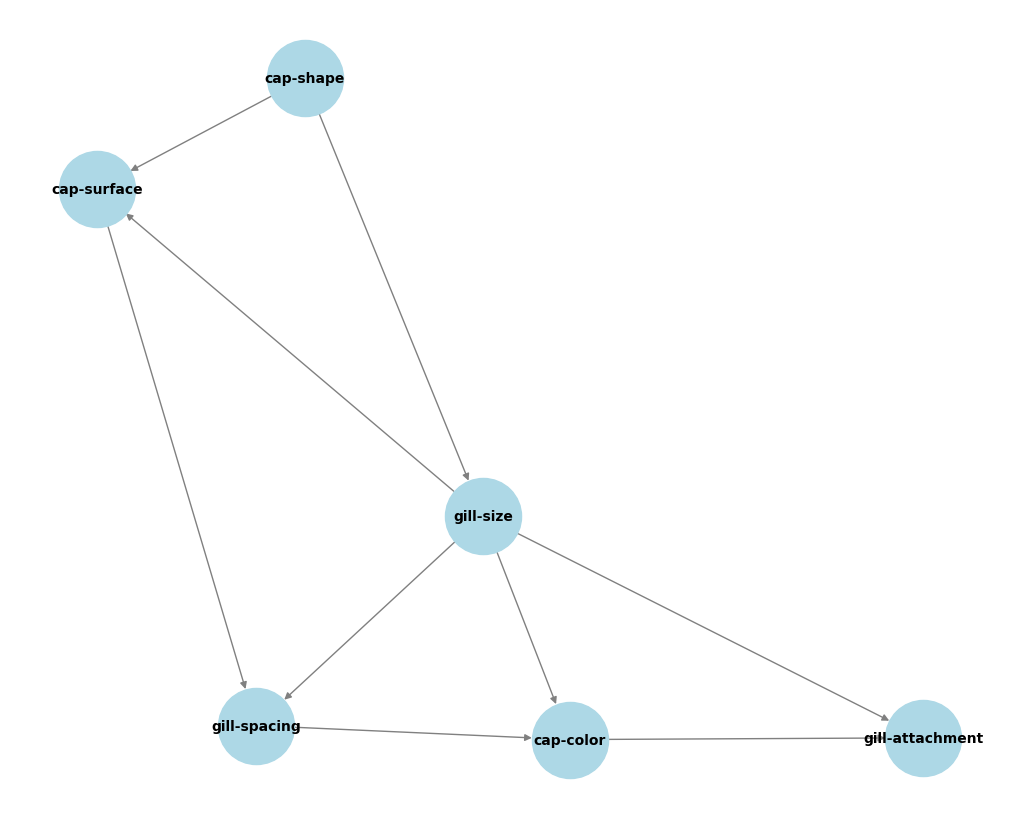
\includegraphics[width=\textwidth]{imgs/betterDAG.png}
\end{subfigure}
\caption{DAG comparison}
\label{fig:DAG comparison}
\end{figure}



\subsection{DINOv2ViT results}
Figure 3 is the best and most recent full training run I achieved with the DINOv2ViT model before I ran out of time and compute credits in Colab. This last run was with the pre-trained DINOv2ViT head, a small number of feature layers, batchnorming, dropout of 0.1, no scheduler, no weighted loss, and a learning rate of 1e-4. My best validation accuracy was $71.52\%$ after epoch 20. Eventually, we can see that the model began to overfit the training set, and accuracy slowly decreased after that point. This validation accuracy shows that 
  \begin{figure}
    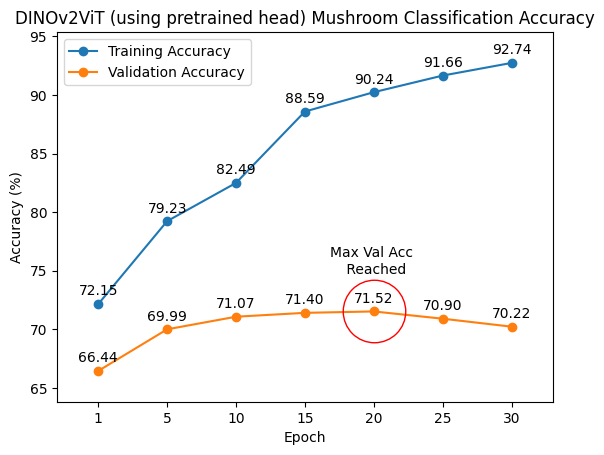
\includegraphics[width=\linewidth]{imgs/Krech_DINOv2ViT_Results_Plot.png}
    \caption{Training and validation set accuracy (percent) results for the DINOv2ViT.}
  \end{figure}

Further, although my benchmark results never technically improved across epochs (which is not surprising given the small set size of the benchmark images), starting even after three epochs, the model achieved four out of six correct classifications.

In conclusion, the DINOv2ViT model results do not look ideal (I certainly would not trust it to decide what mushrooms I should eat or not), but given that the implementation and dataset are limited by our group's and my own limited knowledge and resources, I think it is pretty great! It also had our group's highest validation accuracy percentage at the end of the day. 



\subsection{CNN results}
Figure 4 is the best result I achieved with the CNN model before I ran out of compute. It is clear that despite the measures done to prevent the model from overfitting, it still eventually overfitted, while what it learned was not generalizable. Perhaps an even lower initial learning rate (which was $1e-5$) would prevent overfitting and push the model to generalize on the validation set, which is known to be possible as the results of the DINOv2ViT indicated.
\begin{figure}[H]
    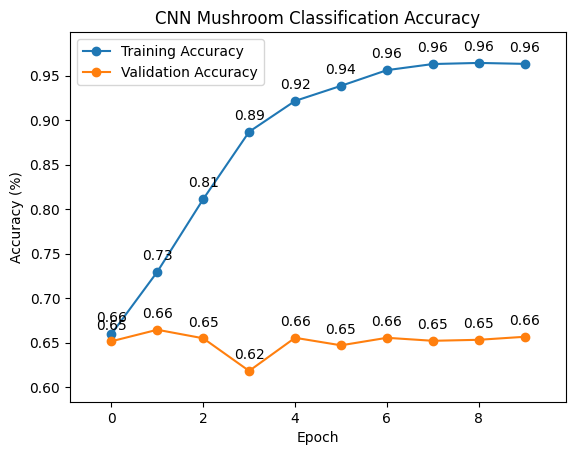
\includegraphics[width=\linewidth]{imgs/cnn_result.png}
    \caption{Training and validation set accuracy (percent) results for CNN.}
\end{figure}
\subsection{LDA results}
One of the drawbacks of using PCA and LDA for classification was the reliance on preprocessing to ensure that the data is suitable for these techniques. In the reference paper, segmentation and gaussian smoothing was used to remove noise from the background. Because of computational limits, I could not add segmentation to the pictures, as segmenting fifty thousand images took many hours. The isolated mushroom images would ensure the subsequent PCA contains relevant components to the mushroom itself, rather than being confounded by backgound or irrelevant noise. As seen in figure 5, PCA did not reduce dimensionality as intended. If the dataset includes background noise, PCA will account for this variance when identifying PC that account for the most variance. This explains why to explain 5303 features were needed to explain 65\% of the variance. This also explains the poor clustering seen in the figure, as noise is not removed. Figure 5 shows the results of PCA where purple represents 0 or 'edible' and yellow represents 1 or 'poisonous'.
\begin{figure}[H]
    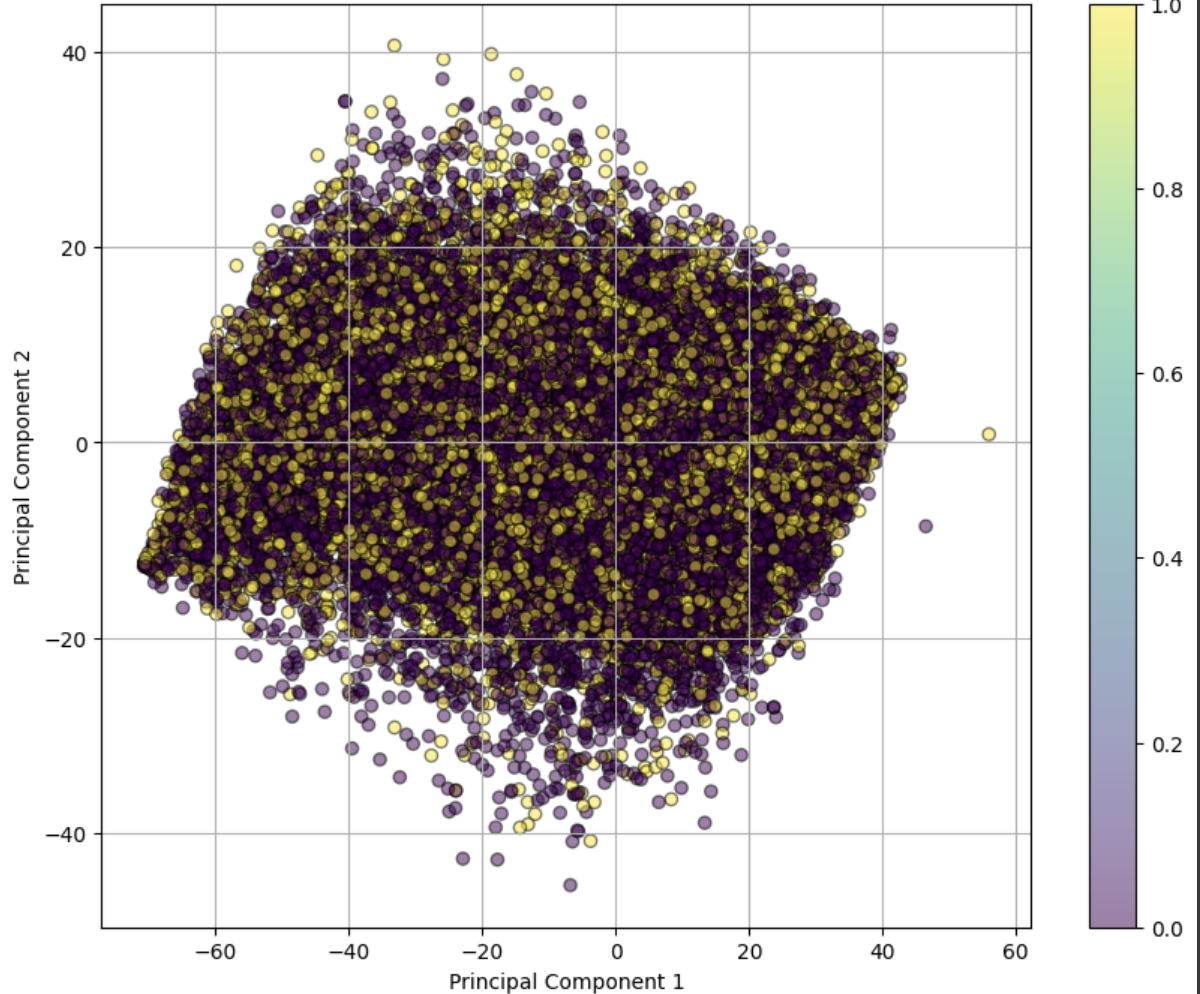
\includegraphics[width=\linewidth]{imgs/pcaplot.png}
    \caption{PCA result data plotted on pc1 and pc2 axis}
\end{figure}
The LDA graph simplifies the representation to one dimension, showing a horizontal layout where edible (purple) clusters towards the left and the poisonous (yellow) towards the right. This indicates the LDA was able to find a discriminant that maximized class separation, however it is not absolute. The model finally achieved an accuracy of 57.19\% accuracy on the validation set, and 70\% on training data. 
\begin{figure}[H]
    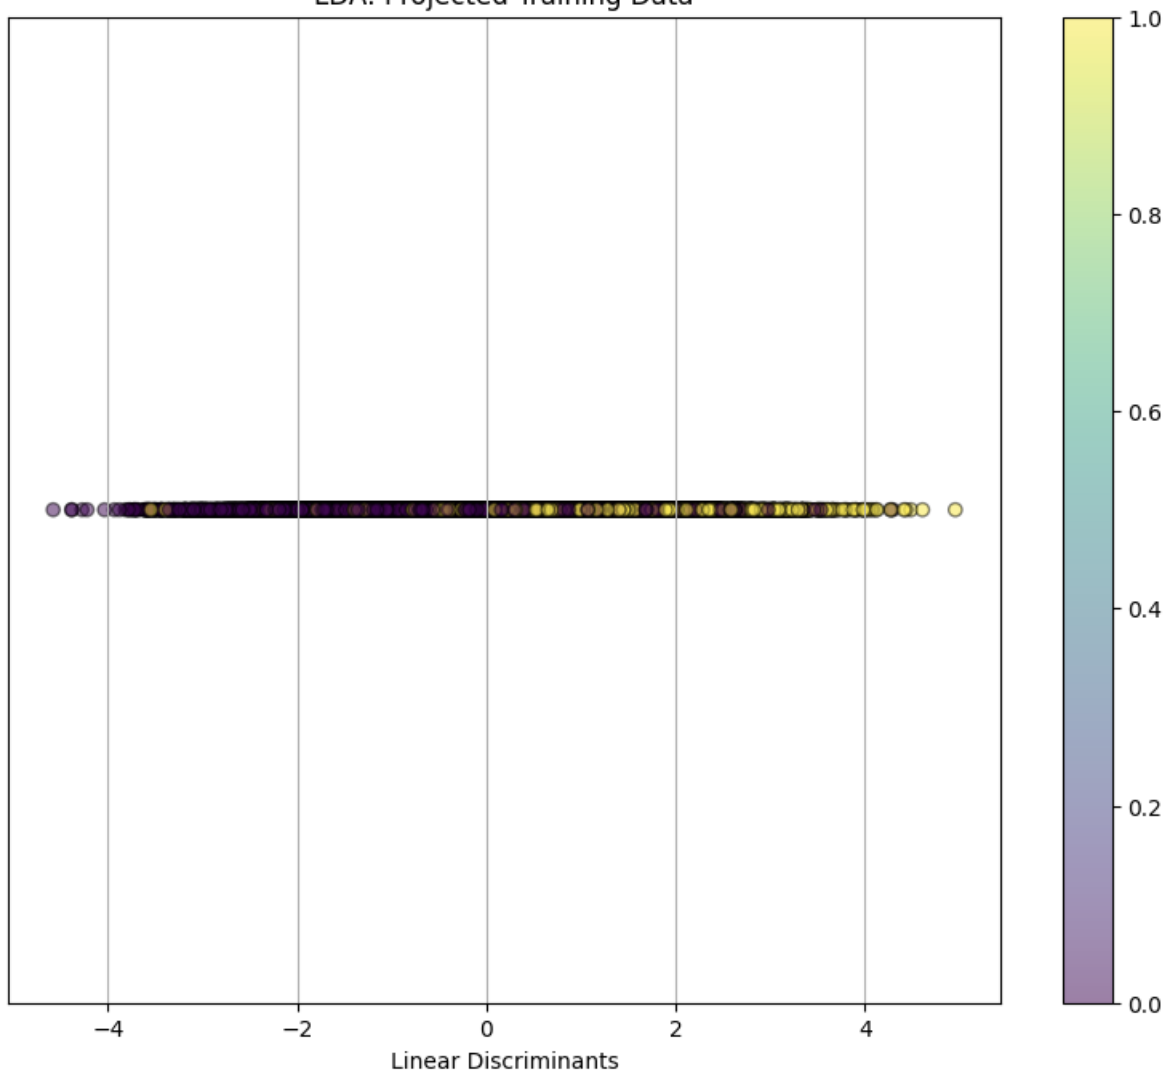
\includegraphics[width=\linewidth]{imgs/ldaplot.png}
    \caption{LDA result on data showing linear separability}
\end{figure}
\section{Conclusion}
At the end of this project we tested 3 neural network based approaches as well as one statistical technique on the mushroom identification problem. By far, the most successful approach was the DINOv2ViT which represents the latest state of art technique and unsurprisingly outperformed CNN, BNN, and LDA. For our 3 neural network approaches, DINOv2ViT classified 4/6 correct while the rest scored 3/6 correct.

However, despite the relatively poor seeming performance of the neural network approaches, we did meet our proposed deliverable goal of creating a model that performs better than chance at identifying mushroom edibility. Considering the standard probability for edible or poisonous is 50/50, we were all technically able to satisfy the requirement of identifying mushrooms at a better rate than random chance; however, it would be very unwise to attempt to apply our approaches to real life sintpatce all of our methods more or less fail the poisonous vs edible look mushroom look-alike test found on the last page. We should also take our data split into account. Even if we used the least balanced set of images (our training set with 64.75\% edible mushrooms), our approaches were all at minimum, reaching that chance level. 

In retrospect, attempting to identify mushrooms from images was an ill-conceived idea because much of the key identifiers of whether a mushroom is poisonous cannot be found from an image, for example: the odor, mushroom bruising, and sporeprint. Our results with maybe the exception of DINOv2ViT once again reaffirm that visual mushroom identification will mainly produce erroneous results but it is the difficult problems that are well worth trying!




\section{Individual Efforts}
Tim handled the BNN portion of the project and experimented on building a Mushroom detection/segmentation pipeline by testing out SAM, FASTSAM, as well as various object detection models. Tim built a custom dataset composed of ~800 images pulled from the site mushsroom.world to train a ResNetv18 to predict categorical mushroom features as there were not any suitable datasets for mushroom identification using categorical features in the public domain. Lastly, Tim also made considerable contributions to the writing of the proposal and report.

Allen labeled and filtered the FGVCx dataset by using a scraper, then built the CNN and MLP classifier and trained it on the FGVCx dataset.

Mikayla utilized a pre-trained DINOv2 as the model encoder and built a vision transformer classifier. I trained it on the FGVCx training dataset Allen provided and tested its accuracy on the validation set. I experimented with scheduling learning rates, weighting the loss functions, batchnorms, dropout rates, and generally adjusting the parameter amount in the model while attempting to improve the accuracy of my model. I compared the speeds of basic CNN and MLP heads in my code as well as comparing the basic ViT and DINO heads to find that the DINO head is a limiting actor in speed, but is still better than the ViT head. Lastly, I tried different torch metrics methods for evalutating performance. 

Namith developed the LDA classifier method for mushroom image classification. This was trained on the labeled and categorized images provided by Allen. I tested different preprocessing techniques to improve the preformance of the classifier, implementing color histograms, SAM segmentation, and edge detection using openCV's canny. 

\begin{figure}[ht]
\centering
\begin{tabular}{ |l|c|c|c|c|c| }
\hline
Mushroom & Expected & BNN & DINO & CNN & LDA\\
\hline
Chanterelle & E & E & & E & \\
\hline
Jack O' Lantern & P & \textcolor{red}{E} & & \textcolor{red}{E} &\\
\hline
Morel & E & E & & E & \\
\hline
False Morel & P & \textcolor{red}{E} & & P &\\
\hline
Shaggy Mane & E & \textcolor{red}{P} & & E &\\
\hline
\specialcell{Green-Spored\\ Parasol} & P & P & & \textcolor{red}{E} & \\
\hline
\end{tabular}
\caption{Classification Benchmarks}
\end{figure}

\begin{figure}[ht]
\centering
\begin{subfigure}[b]{0.45\textwidth}
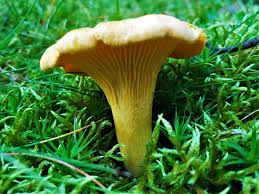
\includegraphics[width=0.3\textwidth]{imgs/chanterelle(double_edible_1).jpg}
\caption{Chanterelle (edible)}
\end{subfigure}
\hfill
\begin{subfigure}[b]{0.45\textwidth}
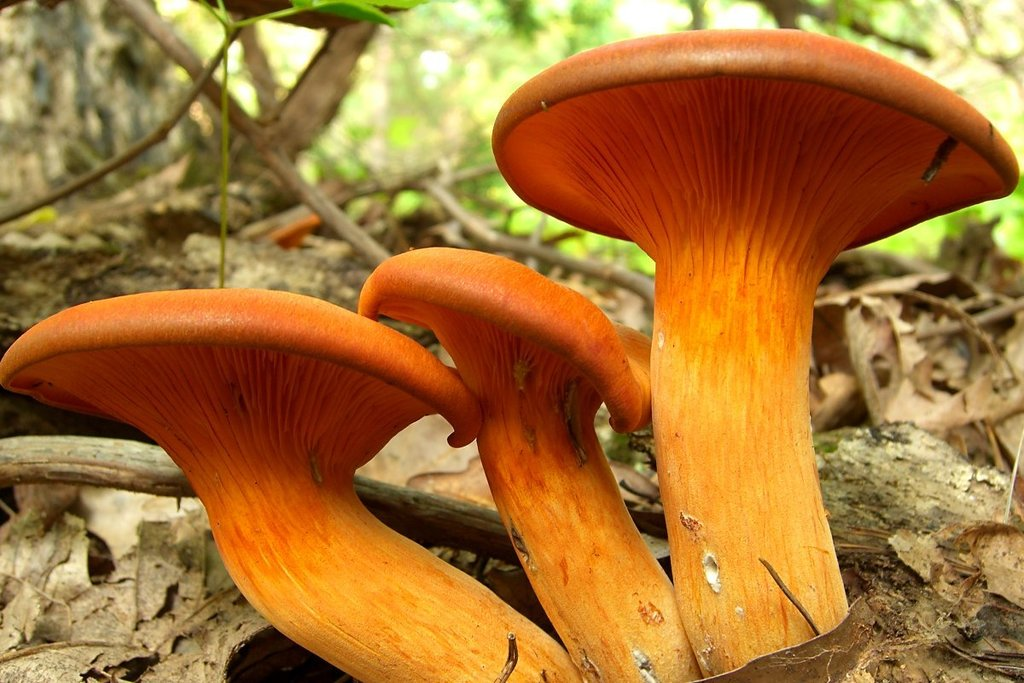
\includegraphics[width=0.3\textwidth]{imgs/jack_o_lantern(double_poisonous_1).jpg}
\caption{Jack O' Lantern (poisonous)}
\end{subfigure}

\medskip
\newpage

\begin{subfigure}[b]{0.45\textwidth}
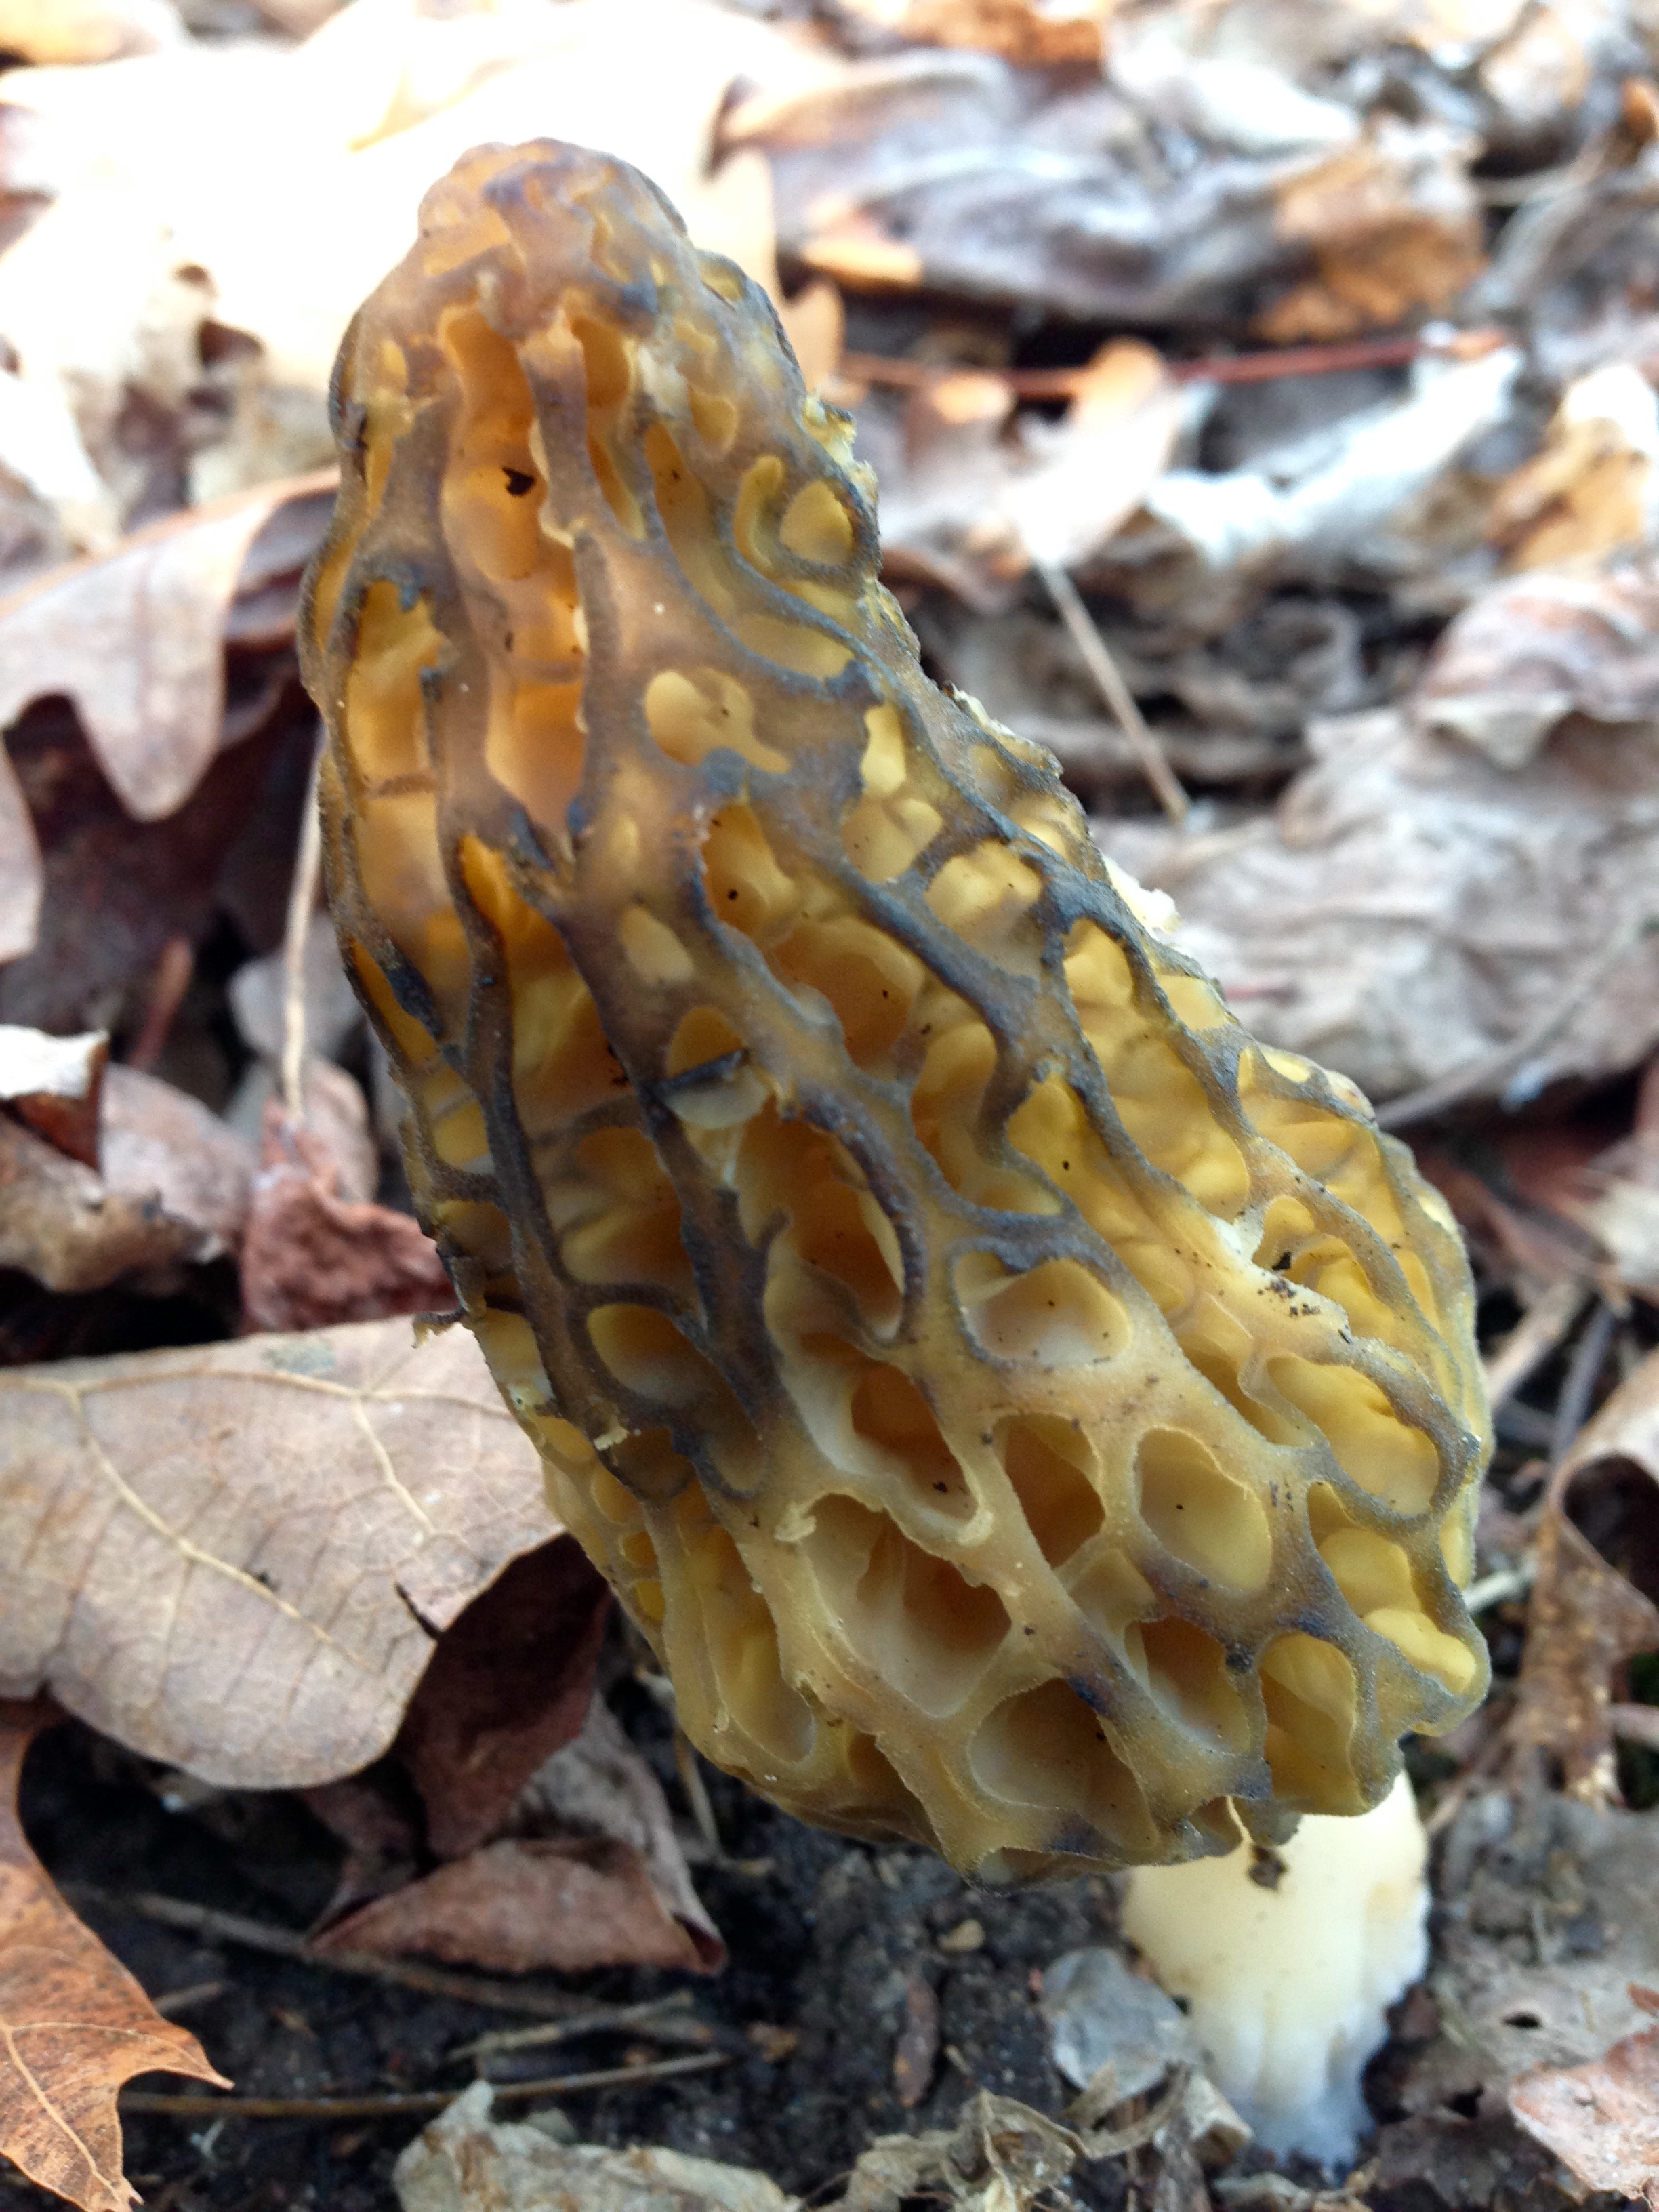
\includegraphics[width=0.3\textwidth]{imgs/morel(double_edible_2).jpg}
\caption{Morel (edible)}
\end{subfigure}
\hfill
\begin{subfigure}[b]{0.45\textwidth}
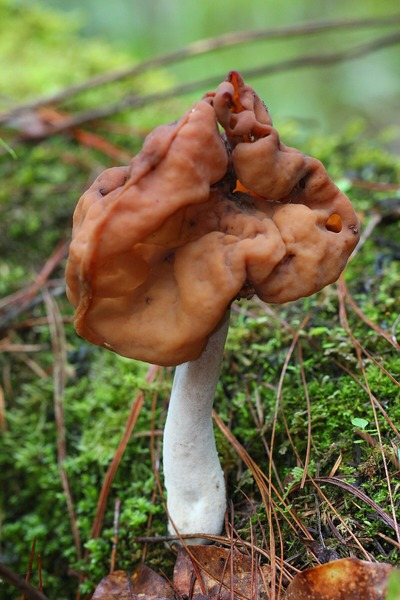
\includegraphics[width=0.3\textwidth]{imgs/false_morel(double_poisonous_2).jpg}
\caption{False Morel (poisonous}
\end{subfigure}

\medskip

\begin{subfigure}[b]{0.45\textwidth}
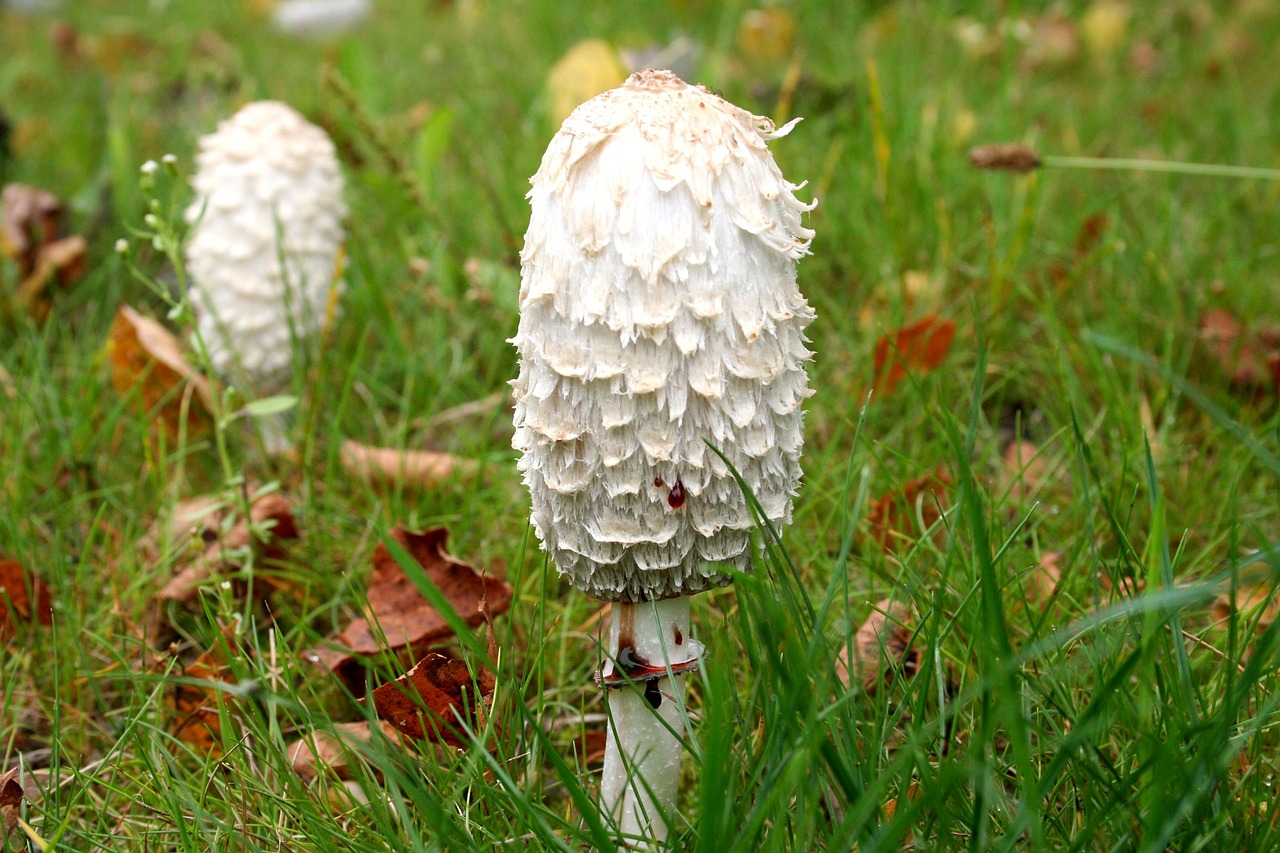
\includegraphics[width=0.3\textwidth]{imgs/shaggy_mane(double_edible_3).jpg}
\caption{Shaggy Mane (edible)}
\end{subfigure}
\hfill
\begin{subfigure}[b]{0.45\textwidth}
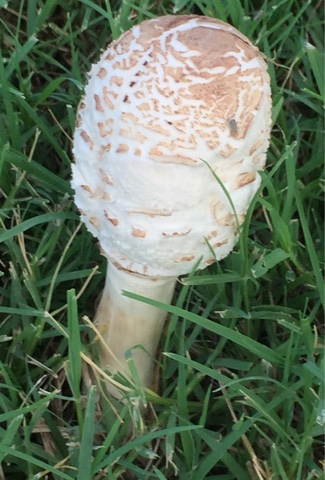
\includegraphics[width=0.3\textwidth]{imgs/green_spored_parasol(double_poisonous_3).jpg}
\caption{Green-Spored Parasol (poisonous)}
\end{subfigure}
\caption{Mushroom Look Alikes}
\label{fig:mushrooms}
\end{figure}


\bibliographystyle{IEEEannot} 
\bibliography{bib}



% biography section
% 
% If you have an EPS/PDF photo (graphicx package needed) extra braces are
% needed around the contents of the optional argument to biography to prevent
% the LaTeX parser from getting confused when it sees the complicated
% \includegraphics command within an optional argument. (You could create
% your own custom macro containing the \includegraphics command to make things
% simpler here.)
%\begin{IEEEbiography}[{\includegraphics[width=1in,height=1.25in,clip,keepaspectratio]{mshell}}]{Michael Shell}
% or if you just want to reserve a space for a photo:

\end{document}

